\subsection*{2.2 Elektrischer Fluss $\Psi$}
    \begin{minipage}{0.49\linewidth}
        \mathbox{
            \Psi = \int \vec{E} d \vec{A}
        }
    \end{minipage}
    \begin{minipage}{0.49\linewidth}
        \begin{scriptsize}
            $E$ = Elektrisches Feld\\
            $A$ = Fläche, durch die das Feld hindurchfliesst
        \end{scriptsize}
    \end{minipage}
    
    \begin{minipage}{0.54\linewidth}
        \begin{empheq}[box = \fbox]{align*}
            \oint \vec{E} \vec{dA} = \frac{1}{\varepsilon_0} \int \rho dV = \frac{Q}{\varepsilon_0}\\
            div(\vec{E}) = \frac{1}{\varepsilon_0} \rho
        \end{empheq}
    \end{minipage}
    \begin{minipage}{0.44\linewidth}
        \begin{scriptsize}
            Mittels dem Satz von Gauss erhält man die erste Maxwell Gleichung\\
            $\rho$ = Ladungsdichte\\
            $Q$ = Gesamtladung innerhalb der Fläche
        \end{scriptsize}
    \end{minipage}

    \subsubsection{Elektrisches Feld Kugel / Punktladung}
        \begin{minipage}{0.39\linewidth}
            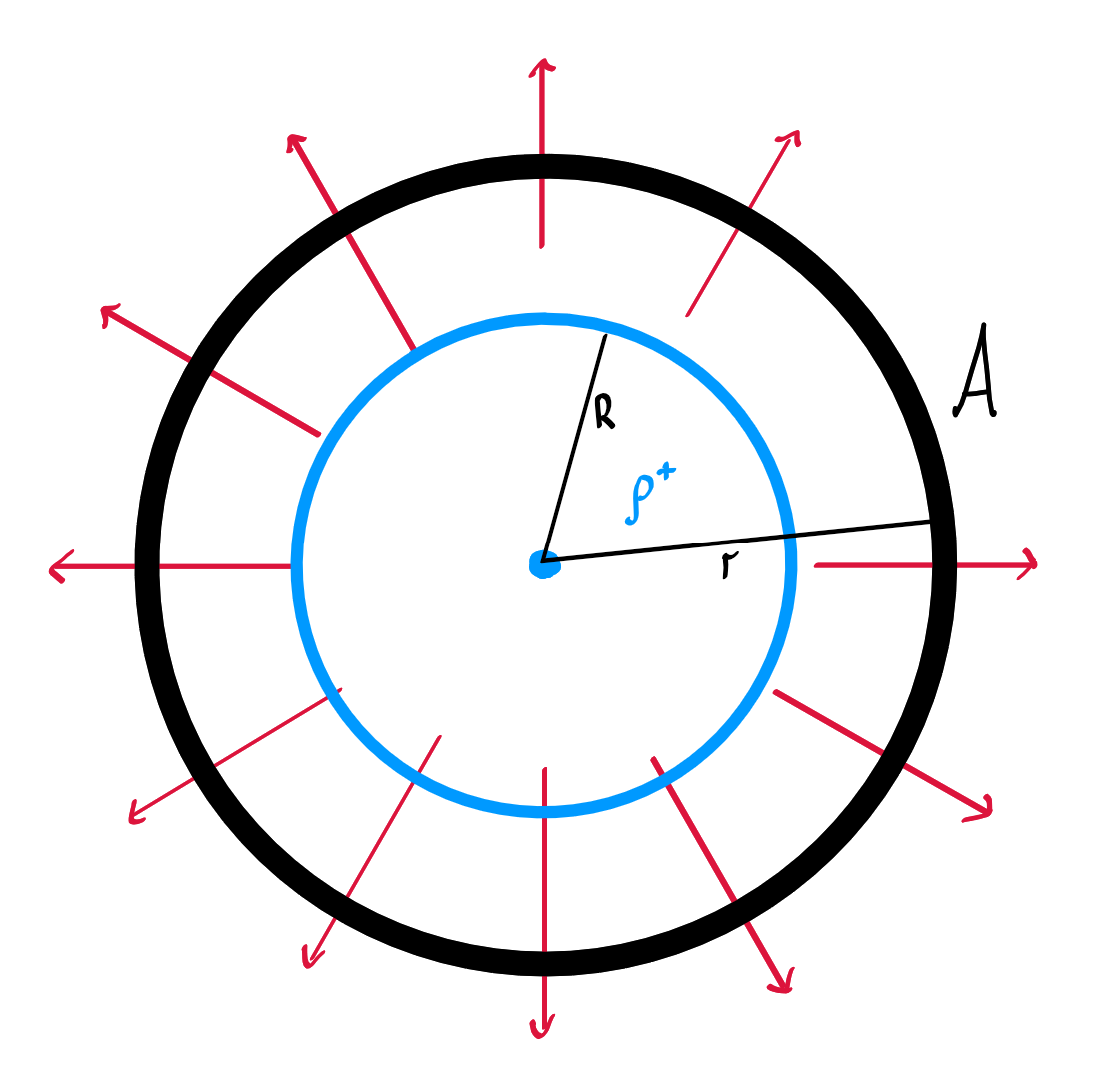
\includegraphics[width = \linewidth]{src/images/e-feld_punktladung.png}
        \end{minipage}
        \begin{minipage}{0.59\linewidth}
            \begin{empheq}{align*}
                &\oint \vec{E} \vec{dA} = \frac{1}{\varepsilon_0} \int \rho dV\\
                r < R \Rightarrow &\vec{E} \cdot 4 \pi r^2 = \frac{\rho \cdot \frac{4}{3} \pi r^3}{\varepsilon_0}\\
                \Aboxed{\Rightarrow & \vec{E} = \frac{\rho r}{3 \varepsilon_0} = \frac{1}{4 \varepsilon_0 \pi } \frac{Q r}{R^3}}\\
                r \geq R \Rightarrow &\vec{E} \cdot 4 \pi r^2 = \frac{\rho \cdot \frac{4}{3}\pi R^3}{\varepsilon_0}\\
                \Aboxed{\Rightarrow & E = \frac{\rho R^3}{3 \varepsilon_0 r^2} = \frac{1}{4 \varepsilon_0 \pi} \frac{Q}{r^2}}\\
                &\rho = \frac{Q}{V} = \frac{3Q}{4 \pi R^3}
            \end{empheq}
        \end{minipage}

    \subsubsection{Elektrisches Feld gerader Leiter}
        \begin{minipage}{0.39\linewidth}
            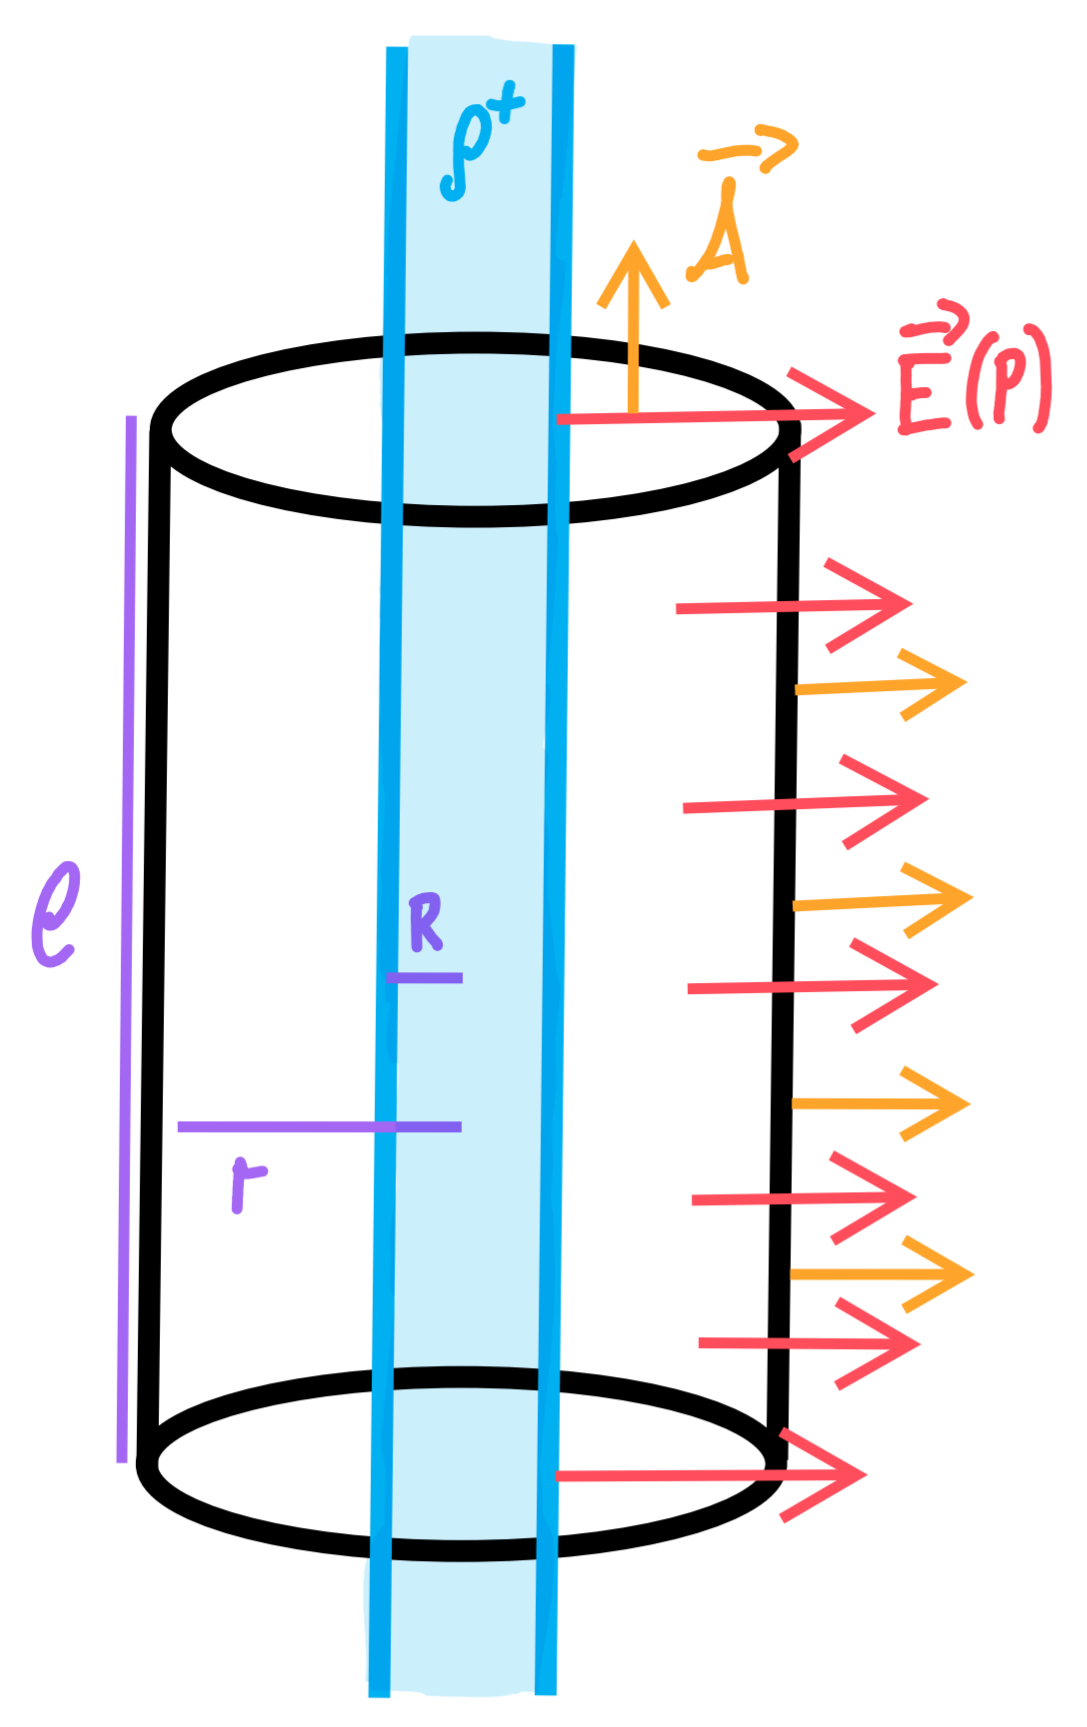
\includegraphics[width = \linewidth]{src/images/e-feld_gerader_leiter.png}
        \end{minipage}
        \begin{minipage}{0.59\linewidth}
            \begin{empheq}{align*}
                &\oint \vec{E} \vec{dA} = \frac{1}{\varepsilon_0} \int \rho dV\\
                r < R \Rightarrow &\vec{E} \cdot 4 \pi r^2 = \frac{\rho \cdot \frac{4}{3} \pi r^3}{\varepsilon_0}\\
                \Aboxed{\Rightarrow & \vec{E} = \frac{\rho r}{3 \varepsilon_0} = \frac{1}{4 \varepsilon_0 \pi } \frac{Q r}{R^3}}\\
                r \geq R \Rightarrow &\vec{E} \cdot 4 \pi r^2 = \frac{\rho \cdot \frac{4}{3}\pi R^3}{\varepsilon_0}\\
                \Aboxed{\Rightarrow & E = \frac{\rho R^3}{3 \varepsilon_0 r^2} = \frac{1}{4 \varepsilon_0 \pi} \frac{Q}{r^2}}\\
                &\rho = \frac{Q}{V} = \frac{3Q}{4 \pi R^3}
            \end{empheq}
        \end{minipage}

    \subsubsection{Elektrisches Feld Platte}
        \begin{minipage}{0.39\linewidth}
            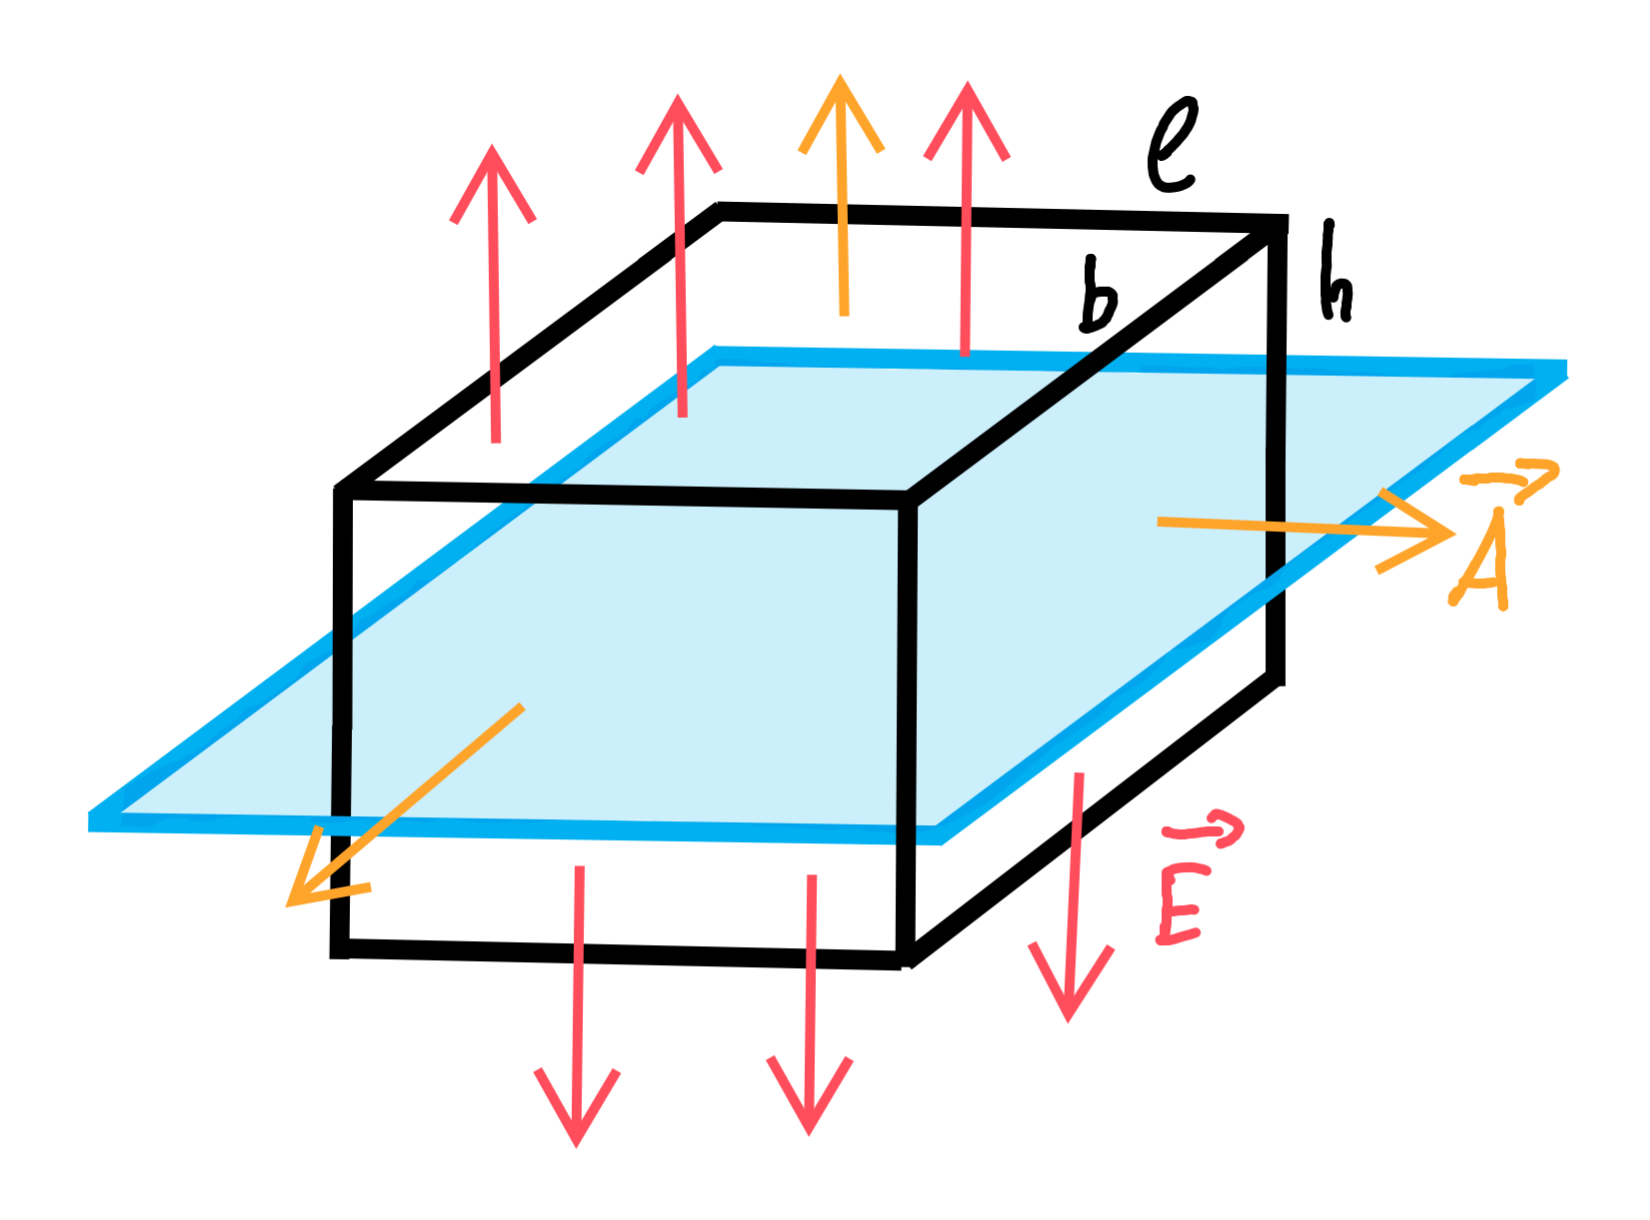
\includegraphics[width = \linewidth]{src/images/e-feld_platte.png}
        \end{minipage}
        \begin{minipage}{0.59\linewidth}
            \begin{empheq}{align*}
                &\oint \vec{E} \vec{dA} = \frac{1}{\varepsilon_0} \int \rho dV\\
                r < R \Rightarrow &\vec{E} \cdot 4 \pi r^2 = \frac{\rho \cdot \frac{4}{3} \pi r^3}{\varepsilon_0}\\
                \Aboxed{\Rightarrow & \vec{E} = \frac{\rho r}{3 \varepsilon_0} = \frac{1}{4 \varepsilon_0 \pi } \frac{Q r}{R^3}}\\
                r \geq R \Rightarrow &\vec{E} \cdot 4 \pi r^2 = \frac{\rho \cdot \frac{4}{3}\pi R^3}{\varepsilon_0}\\
                \Aboxed{\Rightarrow & E = \frac{\rho R^3}{3 \varepsilon_0 r^2} = \frac{1}{4 \varepsilon_0 \pi} \frac{Q}{r^2}}\\
                &\rho = \frac{Q}{V} = \frac{3Q}{4 \pi R^3}
            \end{empheq}
        \end{minipage}
        Für geladene Platten: (Siehe Serie 4 A3) $E = \frac{\rho}{2 \varepsilon_0}$